\documentclass[letterpaper]{article}

\newcommand{\doctitle}{Lab 8: Microbenchmarks and SIMD Instructions}
\newcommand{\docauthor}{Matthew Duschenes}
\newcommand{\docaffil}{Department of Applied Physics, University of Michigan}

\newcommand{\docheader}{NERS 570 - Lab 8 - \docauthor}
\newcommand{\docfooter}{\docaffil}

% Margins
\usepackage[margin=0.75in,marginparsep=0pt,paperwidth=216mm,paperheight=279mm]{geometry}

% Headers
\usepackage{fancyhdr}
\geometry{headheight=15pt}
\renewcommand{\headrulewidth}{0.4pt}% default is 0.4pt
\renewcommand{\footrulewidth}{0.4pt}% default is 0pt
\geometry{headheight=15pt}
\geometry{headsep=10pt}
\setlength{\skip\footins}{10pt} % gap between text and footer
\fancyhf{}
\fancyhead[R]{\docheader}
\fancyfoot[LE,RO]{\thepage}
\fancyfoot[LO,RE]{\docfooter}

% \makeatletter
% \if@twoside
% \fancyfoot[LE,RO]{\thepage}
% \fancyfoot[LO,RE]{\docfooter}
% \else
% \fancyfoot[R]{\thepage}
% \fancyfoot[L]{\docfooter}
% \fi
% \makeatother
% \fancyhead[R]{\docheader}


% Title
\usepackage{titling}
% \usepackage[affil-it]{authblk}
\usepackage[nodayofweek]{datetime}
\usepackage[super]{nth}

% \newdateformat{monthdayyear}{%
%   \monthname[\THEMONTH]~\THEDAY,~ \THEYEAR}
% \newdateformat{mydate}{\monthname[\THEMONTH] \nth[\THEDAY], \THEYEAR}


% Make Title
\pagestyle{fancy}
% \renewcommand*{\Authfont}{\bfseries}
% \renewcommand*{\Affilfont}{\normalfont\itshape}
\pretitle{\begin{center}\vskip -50pt}%
\title{\large \doctitle}
\posttitle{\end{center}}
\preauthor{\begin{center} \vskip -20pt}
\author{}
\postauthor{\end{center} \vskip -20pt}
\predate{\begin{center} \vskip -20pt}
\date{}%\small{\today}}
\postdate{\end{center} \vskip -20pt}% -42.5pt


% Fonts
\usepackage[T1]{fontenc}
\usepackage[singlespacing]{setspace}
\usepackage{dirtytalk}
 
% Math
\usepackage{amsmath}
\usepackage{amssymb}
\usepackage{physics}


% Figures
\usepackage{floatrow}
\usepackage{multicol}
\usepackage{grffile}
\usepackage{caption}
\usepackage{subcaption}
\usepackage{graphicx,xcolor}
\PassOptionsToPackage{export}{adjustbox}

% HypperReferences
\usepackage[pdftex,draft=false]{hyperref}
\hypersetup{
    colorlinks=true,
    linkcolor=black,
    citecolor=black,
    urlcolor=black}
\usepackage{url}

% References
\usepackage[capitalize]{cleveref}


% Code
\usepackage{minted}
\renewcommand\listingscaption{Code}
\floatsetup[listing]{style=Plaintop}    

\crefname{listing}{Code.}{Code}
\newminted{python}{frame=lines,framerule=2pt,float=ht}
\setminted{breaklines,frame=single,framesep=2pt,breakindent=10pt,breakafter={,},breaksymbolleft=}

\newenvironment{longlisting}{\captionsetup{type=listing}}{}
\newcommand{\code}[4]{
% \begin{listing}[ht]
\begin{longlisting}
    \caption{#3}
    \inputminted[linenos]{#1}{#2}
    \label{code:#4}
\end{longlisting}
% \end{listing}
}


 % Commands
\newcommand{\reals}{\mathbb{R}}
\DeclareMathOperator*{\argmax}{arg\,max}
\DeclareMathOperator*{\argmin}{arg\,min}

\newcommand{\eqtxt}[1]{\overset{#1}=}
\newcommand{\repo}[2]{\href{https://github.com/bkochuna/ners570f20-Lab06/#1/#2}{\##2}}


%%%%%%%%%%%%%%%%%%%%%%%%%%%%%%%%%%%%%%%%%%%%%%%%%%%

%%%%%%%%%%%%%%%%%%%%%%%%%%%%%%%%%%%%%%%%%%%%%%%%%%%
\begin{document}

%%%%%%%%%%%%%%%%%%%%%%%%%%%%%%%%%%%%%%%%%%%%%%%
\maketitle
\pagestyle{fancy}
% \singlespacing

%%%%%%%%%%%%%%%%%%%%%%%%%%%%%%%%%%%%%%%%%%%%%%%%



\section{Membench}
The \textit{membench} programs are run to obtain the following plots, from \cref{code:membench}, in \cref{fig:membench_all} to \cref{fig:membench_middle} for the effect of array length and stride length on type of memory access, and time to access. \\ 

In this plot, the solid vertical lines indicate the estimated memory sizes, and dashed vertical lines indicate the true memory sizes, with black lines indicating the cache line sizes, and blue lines indicating the total cache sizes. The green solid horizontal lines indicate the approximate cache access times. \\

In general, it is observed that for a given range of strides, and particularly in regions with plateaus of strides, say between 64B and 4KB, greater array lengths have greater access times. These parallel plateaus can be attributed to filling and then calling the lowest possible caches/accessing the lowest possible level of memory when there are cache misses in the even lower level of memory. This accessing is constant for the given lowest possible memory level. \\

Here, lowest possible memory level refers to the smallest cache at which the stride is less than the cache size and or line size. At this lowest possible level of memory, there will be the least number of cache misses, as it will be assumed that the array will fill this level of cache with as many full cache lines as possible. Larger arrays will fill more cache lines at that level, up to the level being full (and disregarding space being required for the code/instructions on top of space for the data). This filling also depends on whether a cache miss prompts a cache line to be overwritten, or a new cache line to be filled with data from a higher memory level, This depends on the specific association, inclusivity/exclusivity, hierarchy and relative sizes of the different cache levels. \\

So for larger arrays, the number of iterations through the array is obviously greater, and must take more time, and more cache misses will occur, regardless of the relative difference in stride size to cache line size. This greater number of misses (and corresponding new cache lines being filled from higher memory levels) is likely linear in the array size. This linear increase in cache misses explains the parallel plateaus at higher accessing times for greater array sizes, even if the time to access each element within a given cache size is roughly constant. \\

The access times will be measured where there are significant plateaus in the access times, and the \textit{maximum} of these plateaus will be used as an estimate for the access times. The reason there are not sharp increases between plateaus is that as the stride increases, there are less cache hits and more misses as the indexing goes beyond the cache line size, however there are also less indexing calls with greater stride. So the increase up to the next plateau, which corresponds to the memory access time of the next greater memory level, is gradual, as there is a mix of hits in different memory levels. \\

The following script \textit{calc.sh} in the \cref{code:calc} in the appendix was used to get the cpu and memory statistics in \cref{code:cpuinfo}. The average processor core speed for the $36$ processors on GreatLakes to be 3000 MHz, and the cache line sizes appear to be constant at 64 Bytes. The cpu core speed will be used to calculate the number of processor clock cycles required to access the various types of memory, 
$$\textrm{\# cycles per memory access} = \textrm{clock speed}~\times~\textrm{memory access time}.$$

\code{text}{figures/cpuinfo.txt}{CPU and Memory values.}{cpuinfo}

\subsection{Processor Values}
On the Greatlakes compute notes, there are 36 $\times$ Intel(R) Xeon(R) Gold 6140 CPU @ 2.30GHz. From repeated requests for the speed of each core, the average core speed over all cores and samples is 2.99 GHz.

\subsection{$L_1$ Cache Values}
For the $L_1$ cache line size, the true line size is 64B, and from the plots, particularly in \cref{fig:membench_lowerleft}, it can be seen that the access times do not start to initially increase until around strides of 64B, before then plateauing. This jump before plateauing indicates that strides greater than this value must start to involve more $L_1$ misses, and require accessing the $L_2$ memory.
$$ L_1 ~\textrm{Line}~ = 128B. $$

For the $L_1$ total cache size, although the true cache size is 32KB, from the plots, particularly in \cref{fig:membench_lowerleft}, it can be seen that the access times remain very constant, and at their minimum all way the up to 4KB for arrays with length $\leq$ 32KB, suggesting the entire array, or at least half of the array can be loaded into the $L_1$ cache. In addition, the next largest 62KB array shows increased access times for up to 32KB strides, suggesting some $L_1$ cache misses possibly occur, and so the $L_1$ cache size is likely less than 32KB.
$$ 16KB \leq L_1 \leq 32KB. $$

For the $L_1$ access time, given the quite constant access times up to 4KB strides for arrays with length $\leq$ 32KB, the estimated access time is therefore the maximum of the 32KB length array curve:
$$ T_1 = 0.57 \textrm{ns} = 2~\textrm{cycles}.$$





\subsection{$L_2$ Cache Values}
For the $L_2$ cache line size, the true line size is 64B, and from the plots, particularly in \cref{fig:membench_middle}, it can be seen that after the initial increase of access times, there is a slight plateau for strides $\leq$ 512B, and arrays of sizes 64KB-8MB, indicating that possibly the array is being quickly indexed in the $L_2$ cache with a cache line of between 64B and 512B. There is then a jump in access times, but not a huge jump for arrays up to size 8MB, indicating there are possibly still cache hits in the $L_2$ cache, but at different lines.
$$ 64B \leq L_2 ~\textrm{Line}~ \leq 512B. $$


For the $L_2$ total cache size, although the true cache size is 1MB, from the plots, particularly in \cref{fig:membench_middle}, it can be seen that the access times remain very constant over a large range of array sizes between 64KM to 8MB, with strides between 1KB and 256KB. This suggests lots of these array sizes can be mostly loaded into the $L_2$ cache on several cache lines. This suggests the $L_2$ total cache size to be less than 256KB (and greater than the $L_1$ total cache size); the point where the access times for these array sizes drops dramatically when many less array elements are indexed. The difficulty at finding tighter bounds on the $L_2$ cache sizes is possibly due to the $L_2$ cache sometimes being shared by pairs of cores, affecting the timing, depending on which cores the array is being computed on.
$$ 16KB \leq L_2 \leq 256KB. $$

For the $L_2$ access time, given the quite constant access times for array sizes between 64KM to 8MB, with strides between 1KB and 256KB, the estimated access time is therefore the maximum of the 8MB size array curve along this plateau:
$$ T_2 = 3.83 \textrm{ns} = 12~\textrm{cycles}.$$



\subsection{$L_3$ Cache Values}
For the $L_3$ cache line size, the true line size is 64B, however from the plots, it is difficult to tell where exactly there is a distinct plateau for array indexing with strides within the size of this larger cache's lines. This may be due to the $L_3$ cache being typically shared between all (36) cores, and so timings may be affected depending how the computations are distributed amongst the cores. However for array sizes of 16MB to 512MB, there is somewhat a plateau between 512B and 4KB, indicating a possible range for the $L_3$ cache line size. Here, there may be hits due to this larger cache being allowed to store more of these larger arrays, minimising cache misses. The lack of distinct plateau is also possibly attributed to the large arrays being far larger than the cache, and there being many hits and misses while the lines are being filled from the main memory.
$$ 64B \leq L_3 ~\textrm{Line}~ \leq 4KB. $$

For the $L_3$ total cache size, although the true cache size is 24.75MB, from the plots, particularly in \cref{fig:membench_middleupper}, it can be seen that the plateau between 512B and 4KB, for array sizes of 16MB to 512MB, rises, and then decreases gradually, before plateauing again for strides between 256KB and 8MB. This suggests that the time is not decreasing solely due to there being less elements indexed with greater stride, but there also possibly being effects of the elements still being in the faster $L_3$ cache compared to the main memory. There are still hits occurring in succession in a cache that are causing this plateau at non-zero access times. There is still though great uncertainty in the exact total size of this $L_3$ cache.
$$ 256KB \leq L_3 \leq 8MB. $$

For the $L_3$ access time, given the two different plateaus present in the access times for the larger arrays, the access time will be estimated as the maximum of these plateaus in \cref{fig:membench_middleupper}.
$$ T_3 = 10.36 \textrm{ns} = 32~\textrm{cycles}.$$


\subsection{Main Memory Values}
Only the 1GB array sizes appear to be unable to be stored fully in any caches, and there are enough misses in the lower caches that the main memory must be accessed. It is assumed the upper plateau for the 1GB array are these memory hits, and the access time is assumed to be the maximum of this plateau. This is assumed to be a lower bound, if some of the array is in the $L_3$ cache, and there are some hits there, and some in the main memory.

$$ T_{\textrm{mem}} \geq 13.69 \textrm{ns} = 42~\textrm{cycles}.$$




\begin{figure}[H]
  \centering
  %  trim={<left> <lower> <right> <upper>}
  % \captionsetup{skip=-12pt,format=hang}
  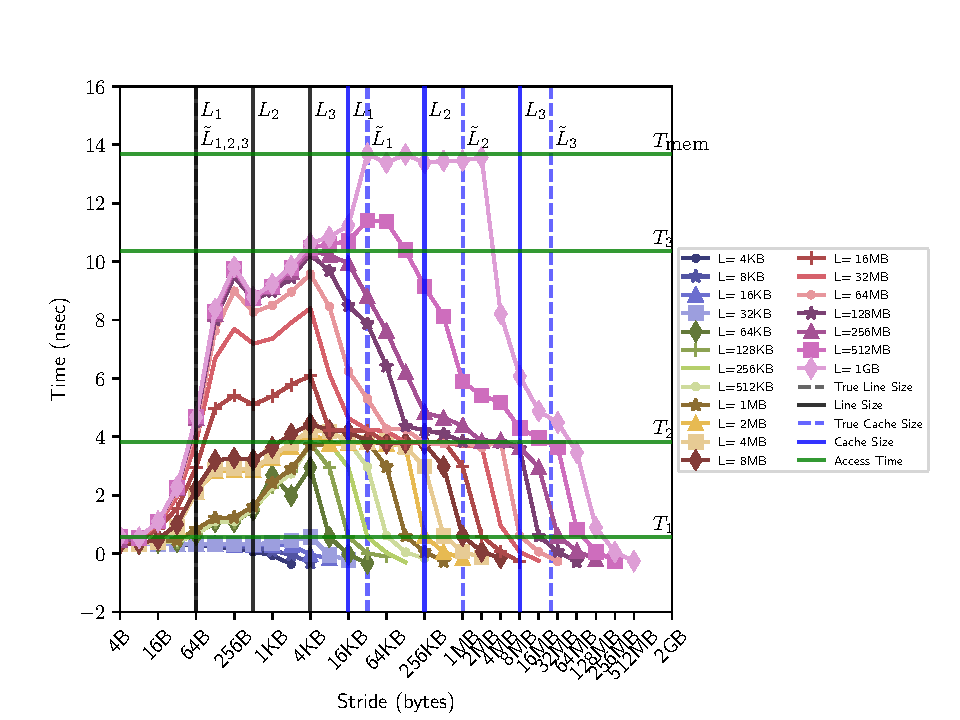
\includegraphics[width=\textwidth]{figures/membench_all.pdf}
  % \vspace{-8pt}
  \caption{Memory access times for various array sizes, and stride lengths from 4B to 512MB.}
  \label{fig:membench_all}
\end{figure}

\begin{figure}[H]
  \centering
  %  trim={<left> <lower> <right> <upper>}
  % \captionsetup{skip=-12pt,format=hang}
  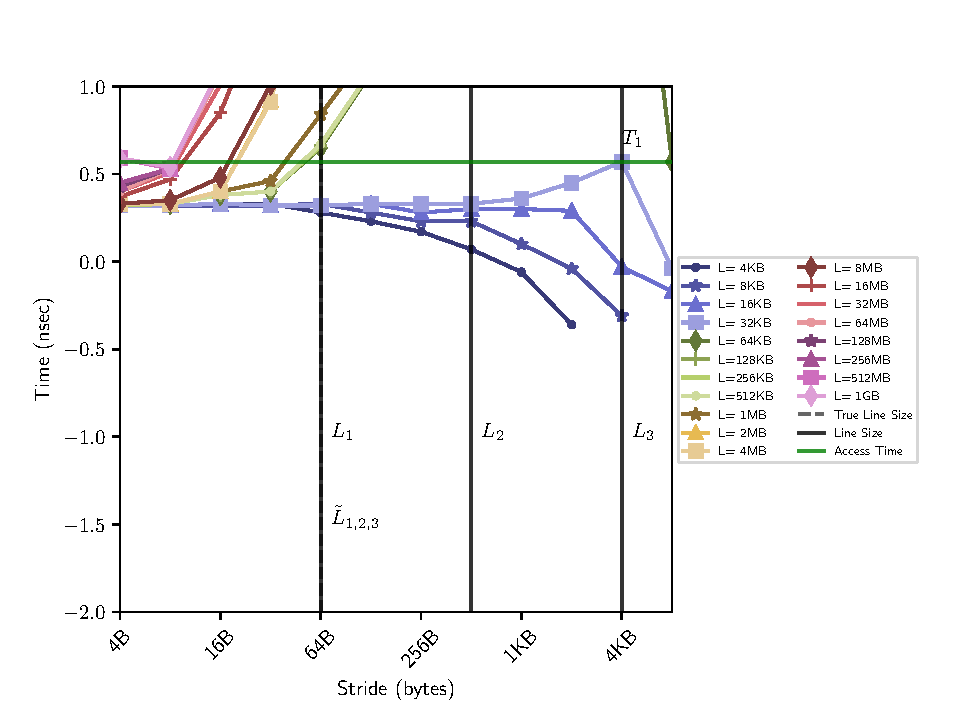
\includegraphics[width=\textwidth]{figures/membench_lowerleft.pdf}
  % \vspace{-8pt}
  \caption{Memory access times for various array sizes, and stride lengths from 4B to 4KB.}
  \label{fig:membench_lowerleft}
\end{figure}


\begin{figure}[H]
  \centering
  %  trim={<left> <lower> <right> <upper>}
  % \captionsetup{skip=-12pt,format=hang}
  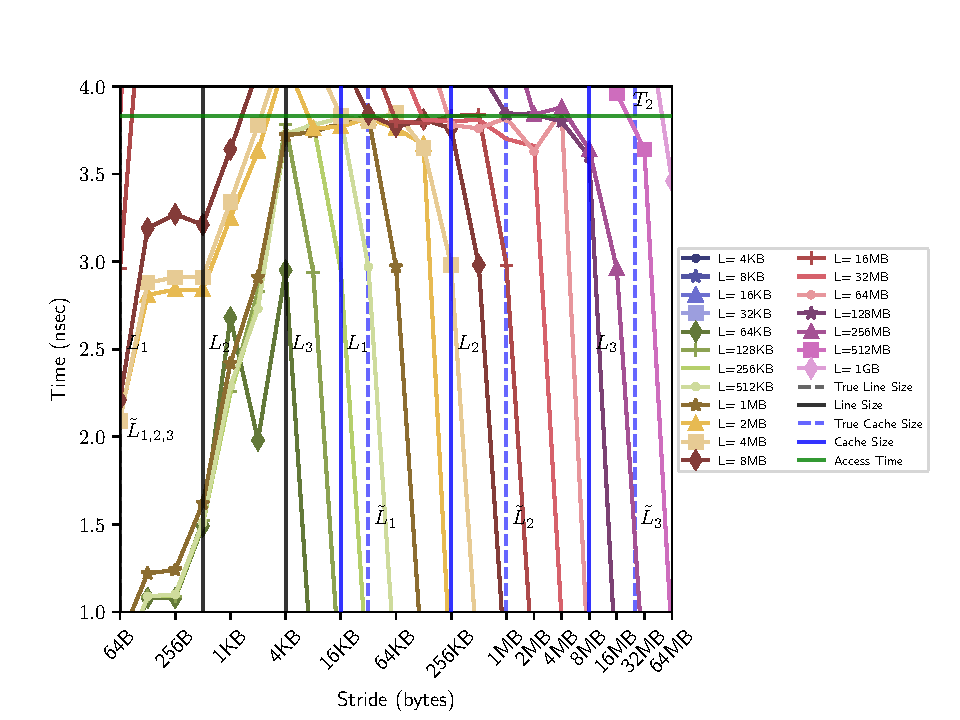
\includegraphics[width=\textwidth]{figures/membench_middle.pdf}
  % \vspace{-8pt}
  \caption{Memory access times for various array sizes, and stride lengths from 16B to 64MB.}
  \label{fig:membench_middle}
\end{figure}


\begin{figure}[H]
  \centering
  %  trim={<left> <lower> <right> <upper>}
  % \captionsetup{skip=-12pt,format=hang}
  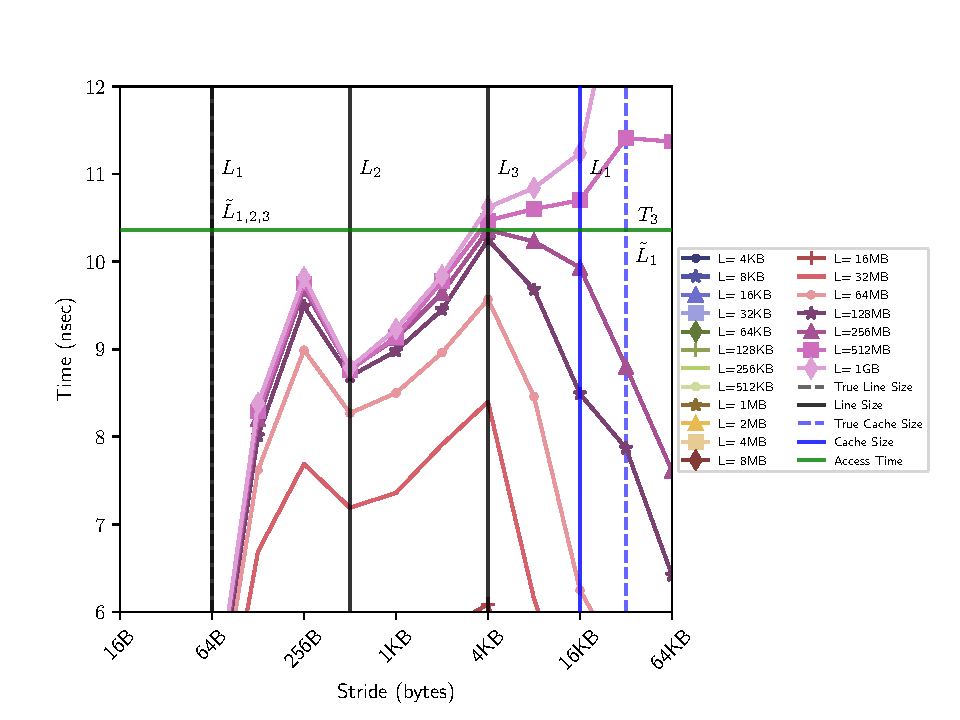
\includegraphics[width=\textwidth]{figures/membench_middleupper.pdf}
  % \vspace{-8pt}
  \caption{Memory access times for various array sizes, and stride lengths from 16B to 64KB.}
  \label{fig:membench_middleupper}
\end{figure}


\newpage
\section{SIMD Instructions}

\subsection{AVX Support}
\begin{itemize}
	\item The commands used to verify if the current machine/processor supports AVX are:
	$$ \textrm{grep -E \say{avx[\^{}0-9]} /proc/cpuinfo}$$
	and if the current machine/processor supports AVX2 are:
	$$ \textrm{grep -E \say{avx2} /proc/cpuinfo}$$ 

	These searches will show whether the supported AVX fields are in the flags section of the processor info from /proc/cpuinfo. This command will show all processors (36 $\times$ Intel(R) Xeon(R) Gold 6140 CPU @ 2.30GHz, for GreatLakes compute nodes).
	
	\item The commands used to verify if the current GNU compiler supports AVX or AVX2 by the constants/macros the compiler defines:
	$$ \textrm{gcc -mavx2 -dM -E - < /dev/null | grep "AVX" | sort } $$
	This command will show the boolean settings for the AVX constants:\\
	\#define \_\_AVX\_\_ 1 \\
	\#define \_\_AVX2\_\_ 1 \\
	
	\item The commands used to verify if the current Intel compiler supports AVX or AVX2 by the constants/macros the compiler defines:
	$$\textrm{ icc -march=native -dM -E - < /dev/null | grep "AVX" | sort } $$
	This command will show the boolean settings for the AVX constants:\\
	\#define \_\_AVX\_\_ 1 \\
	\#define \_\_AVX2\_\_ 1 \\
	\#define \_\_AVX512BW\_\_ 1 \\
	\#define \_\_AVX512CD\_\_ 1 \\
	\#define \_\_AVX512DQ\_\_ 1 \\
	\#define \_\_AVX512F\_\_ 1 \\
	\#define \_\_AVX512VL\_\_ 1 \\
	\#define \_\_AVX\_I\_\_ 1 \\
\end{itemize}

\subsection{dgemm Assembly Instructions}
The command to get the assembly instructions is as follows, where the function for the naive \textit{dgemm.cpp} in \cref{code:dgemm} in the appendix is translated into assembly code, with the avx2 and fast optimizations using the commands for gnu and intel compilers:
$$\textrm{g++ -S -Ofast -mavx2 -mfma dgemm.cpp} $$ \\
$$\textrm{icc -S -Ofast -march=core-avx2 dgemm.cpp} $$ \\


This command (with the gnu compiler) produces the following assembly code in \cref{code:asb}. Here it can be seen in lines 81-120, there is the assembly code for the three loops (add, \textit{add},compute, \textit{cmp}, jump, \text{jne}, as well as the vectorized multiply \textit{vmulsd}, add \textit{add}, and vectorized move \textit{vmovsd}. The specific SIMD fused multiply-add commands are \textit{vfmadd132sd}. \\

The assembly instructions are known to contain AVX2 instructions because they are writing to the AVX specific register keywords \textit{ymm}, and AVX2 is confirmed, because fused-multiply-add commands (such as \textit{vfmadd132sd}) are in the assembly instructions.\\

Considering the correct compiler options and hardware compatibility for AVX2 instructions has appeared to be verified, no modifications of the original matrix-matrix multiplication source code were necessary. The mydgemm, compiled with the above avx2 and fma options, as well as the fast optimizations, does not appear on GreatLakes to run faster, at least for matrix sizes up to 2000.


\begin{longlisting}
    \caption{Matrix-matrix multiplication loop assembly code}
    \inputminted[linenos,firstline=81,lastline=120]{bash}{figures/dgemm.s}
    \label{code:asb_}
\end{longlisting}


\code{cpp}{figures/dgemm.s}{Matrix-Matrix multiply assembly with avx2 and fast optimization}{asb}






\newpage
\section{In-line Assembly}
With help from the internet, the following matrix-vector multiplication $y=Ax$, in-line assembly,as well as conventional c code, is shown in \cref{code:matvec} in the appendix. The fused-multiply adds assembly was not quite able to be implemented, however the procedure of writing the fused-multiply adds with avx instructions (in the assembly syntax, as opposed to the intel syntax) was attempted. There are no compiler errors, however the issue seems to be that the $y$ value is not being assigned the computed multiplied value in the set register in \textit{\_mm\_storel\_pd(y, \_mm256\_castpd256\_pd128(Ax))}.

The assembly registers for multiplies and adds currently only allow for operating on $4\times4$ matrices if double precision is used. So, blocks of the matrix and vector in these sizes must be passed to the assembly function \textit{\_matvec\_avx(A,x,y)} in a loop. This loop can then be unrolled, to assign each part of $y$ separately. 

The program is compiled with the following command, and assembly snippet is shown in \cref{code:matvec_asm}.
$$\textrm{gcc -Ofast -mavx2 -mfma -funroll-all-loops matvec.c} $$ \\


\begin{longlisting}
    \caption{Matrix-Vector multiplication inline assembly code}
    \inputminted[linenos,firstline=202,lastline=234]{c}{figures/matvec.c}
    \label{code:matvec_asm}
\end{longlisting}












\newpage
\section{Appendix}
\appendix
\begin{appendix}
\code{python}{figures/membench.py}{membench plotting script.}{membench}
\newpage
\code{bash}{figures/calc.sh}{CPU Info script.}{calc}
\newpage
\code{bash}{figures/job.slurm}{membench job script.}{job}
\newpage
\code{cpp}{figures/dgemm.cpp}{Matrix-Matrix multiply}{dgemm}
\newpage
\code{c}{figures/matvec.c}{Matrix-Vector multiply}{matvec}
\end{appendix}


%%%%%%%%%%%%%%%%%%%%%%%%%%%%%%%%%%%%%%%%%%%%%%%%
\end{document}